\documentclass[a4paper,12pt,bibliography=totoc, listof=totoc, titlepage]{scrreprt}
\usepackage[T1]{fontenc}
\usepackage{lmodern}
\usepackage[british,ngerman]{babel}
\usepackage[babel]{microtype}
\usepackage[utf8]{inputenc}
\usepackage[left=2.5cm,right=3cm,top=2.5cm,bottom=2.5cm]{geometry}
\usepackage[onehalfspacing]{setspace}
\renewcommand{\arraystretch}{1.5}
\usepackage{graphicx}
\graphicspath{{img/}}
\usepackage[dvipsnames,table,xcdraw]{xcolor}
\usepackage[toc,page]{appendix}
\usepackage[printonlyused]{acronym}

\usepackage{pdfpages}
%\usepackage[scaled]{berasans}
%\renewcommand*\familydefault{\sfdefault}  %% Only if the base font of the document is to be sans serif

% Absatz-Einstellungen
\setlength{\parindent}{15pt} % Einrücken
\setlength{\parskip}{6pt}  % Horizontaler Abstand

\usepackage{subcaption}
\usepackage{graphicx} % omit 'demo' for real document
  
\usepackage[hyphens]{url}
\usepackage[colorlinks=true,allcolors=BlueViolet]{hyperref}
\setlength {\marginparwidth }{2cm}
\usepackage{todonotes}
\usepackage{amsmath}
\usepackage{siunitx}
\sisetup{locale = DE}
\usepackage{icomma}
\newcommand\nlabel[1]{\addtocounter{equation}{1}\tag{\theequation}\label{#1}}

\usepackage{cancel}
\usepackage{scrhack}
\usepackage{scrtime}
\usepackage{enumitem}

\usepackage[headsepline,automark]{scrlayer-scrpage}
\clearpairofpagestyles
\ihead{\headmark}
\cfoot*{\pagemark}
\pagestyle{scrheadings}


% Kommentare mit \begin{comment}
\usepackage{verbatim}

\usepackage{multirow}

\newcommand*\justify{%
  \fontdimen2\font=0.4em% interword space
  \fontdimen3\font=0.2em% interword stretch
  \fontdimen4\font=0.1em% interword shrink
  \fontdimen7\font=0.1em% extra space
  \hyphenchar\font=`\-% allowing hyphenation
}


\usepackage{tablefootnote} % for table footnotes

\usepackage{array,tabularx,calc}

\newlength{\conditionwd}
\newenvironment{conditions}[1][mit]
  {%
   #1\tabularx{\textwidth-\widthof{#1}}[t]{
     >{$}l<{$} @{${}:{}$} X@{}
   }%
  }
  {\endtabularx\\[\belowdisplayskip]}

\newcommand{\code}[1]{\texttt{\justify{#1}}}
%\usepackage{tocloft}

%Boxfehler
\hfuzz=1pt
\hbadness=1000000

% Hurenkinder und Schusterjungen verhindern
\clubpenalties 5 10000 10000 10000 1000 1000
\widowpenalties 5 10000 10000 10000 1000 1000
\displaywidowpenalty=10000


% Zitierstil
%\usepackage[style=authoryear,citestyle=authoryear,natbib=true]{biblatex}
%\bibliography{Thesis.bib}
\usepackage[round]{natbib}
\bibliographystyle{hcu}
\def\biblio{
    \ifSubfilesClassLoaded{%
        \nocite{timm}
        \printglossaries
        \bibliography{./00PhotoBox}
        \listoffigures
        \listoftables
    }{}
}

\usepackage[acronym, toc]{glossaries}

\makeglossaries

\loadglsentries{99Glossar.tex}
\usepackage{{booktabs}}


\usepackage{subfiles}

\title{Aufbau eines photogrammetrischen Messsystems mit Raspberry-Pi-Kameras als Low-Cost-Sensoren für die Aufnahme von kleinen Objekten}
\author{Florian Timm}
\date{November 2024}


\begin{document}
\def\biblio{}
\pagenumbering{Roman}
\begin{titlepage}
    \begin{center}
        \renewcommand{\arraystretch}{0.7}
        \renewcommand{\baselinestretch}{1.5}
        \begin{tabular}{lr}
            \begin{tabular}{l}
                
\includegraphics[width=0.35\textwidth]{img/hculogo_grau.png}
            \end{tabular} \hspace{1.2cm} &
            \begin{tabular}{r}
                Universität für           \\Baukunst und Metropolenentwicklung\\
                Henning-Voscherau-Platz 1 \\
                20457 Hamburg             \\
            \end{tabular}
        \end{tabular}\\\vspace{4cm}

        {\huge\bfseries Aufbau eines\\photogrammetrischen Messsystems\\mit Raspberry-Pi-Kameras als\\Low-Cost-Sensoren\\}
        {\LARGE\bfseries für die Aufnahme von kleinen Objekten\\}~\vspace{0.5cm}\\

        {\large\bfseries Geodäsie und Geoinformatik\\Masterthesis\\Sommersemester 2024}\vspace{2cm}\\
        {\large Florian Timm}

        % hspace und vspace bedeutet horizontaler bzw. vertikaler Abstand
        \vspace{3cm}
        Abgabedatum: 28. Oktober 2024 \\
        mit Korrekturen vom 10. Januar 2025
    \end{center}
    \setcounter{page}{0} % Seitenzahl wird auf 0 gesetzt 
\end{titlepage}

\KOMAoption{headsepline}{false}
\vspace{1cm}
\noindent\textbf{\large Verfasser}\\
Florian Timm\\
Matrikelnummer: 6028121\\
Gaiserstraße 2, 21073 Hamburg\\
\\
E-Mail: florian.timm@hcu-hamburg.de / info@florian.timm.de \\
\vspace{2cm}\\
\noindent\textbf{\large Erstprüfer}\\
Prof. Dr.-Ing. Thomas Kersten\\
HafenCity Universität Hamburg\\
Henning-Voscherau-Platz 1, 20457 Hamburg\\
\\
E-Mail: thomas.kersten@hcu-hamburg.de\\
\vspace{2cm}\\
\textbf{\large Zweitprüfer}\\
Dipl.-Ing. Kay Zobel\\
HafenCity Universität Hamburg\\
Henning-Voscherau-Platz 1, 20457 Hamburg\\
\\
E-Mail: kay.zobel@hcu-hamburg.de\\
\vspace{4cm}\\
Sofern keine andere Quelle in der Bildunterschrift genannt wird, handelt es sich bei den Abbildungen um eigene Darstellungen. Diese dürfen unter Namensnennung weiterverwendet werden.
\newpage
\begin{abstract}
    \noindent\textbf{\large Kurzzusammenfassung}\\
    Die Photogrammetrie ermöglicht die Erstellung von 3D-Modellen unter Zuhilfenahme relativ einfacher Technik. Allerdings ist der Zeitaufwand für die Aufnahme der Bilder oft hoch, sodass sich diese Methode nicht für die Erfassung einer großen Anzahl von Objekten eignet, beispielsweise für die Digitalisierung von Museumsbeständen. Systeme, die auf mehreren fest installierten Kameras basieren, verwenden in der Regel hochwertige Kameras. Dies führt jedoch zu einem signifikanten Anstieg der Hardwarekosten.

    Im Rahmen dieser Arbeit erfolgt eine Untersuchung des Lösungsansatzes, mehrere kostengünstige Kameras zu verwenden, die fest auf einem Rahmen montiert sind. Den Kern dieser Untersuchung bildet der Aufbau eines photogrammetrischen Messsystems für kleine Objekte, welches aus Raspberry-Pi-Kameras besteht. Im Rahmen der Entwicklung ist die Programmierung einer Schnittstelle zur Synchronisation der Kameras sowie die Entwicklung einer Möglichkeit zur Kalibrierung der Kameras vorgesehen. In einem nächsten Schritt wird die Genauigkeit der Erfassung überprüft. Das Endergebnis soll im Idealfall einem photogrammetrischen Laien ermöglichen, schnell und ohne lange Einarbeitungszeit 3D-Modelle in ausreichender Auflösung und Qualität zu erzeugen.

    \vspace{2cm}
    \begin{otherlanguage*}{british}
        \noindent\textbf{\large Abstract}\\
        Photogrammetry enables the creation of 3D models using relatively simple technology. However, the time required to capture the images is often high, meaning that this method is not suitable for capturing numerous objects, for example when digitizing museum collections. Systems based on several permanently installed cameras generally use high-quality cameras. However, this results in a significant increase in hardware costs.

        This thesis investigates the solution of using several low-cost cameras mounted on a fixed frame. The core of this investigation is the construction of a photogrammetric measurement system for small objects, which consists of Raspberry Pi cameras. The programming of an interface to synchronize the cameras and the development of a way to calibrate the cameras are planned as part of this. The next step will be to check the accuracy of the recording. Ideally, the end result should also enable a photogrammetric layman to generate 3D models in acceptable resolution and quality quickly and without a long familiarization period.
    \end{otherlanguage*}
\end{abstract}
\newpage
\KOMAoption{headsepline}{true}

\tableofcontents
\newpage

\pagenumbering{arabic}
\setcounter{page}{1}

\subfile{01Einleitung}

\subfile{02Grundlagen}

\subfile{03Aufbau}

\subfile{04Voruntersuchungen}

\subfile{05Software}

\subfile{06Kalibrierung}

\subfile{07Versuche}

\subfile{08Fazit}

\clearpage

\printglossaries

\clearpage
%Literatur
\renewcommand\UrlFont\itshape
\renewcommand{\refname}{Literaturverzeichnis}
\bibliography{00PhotoBox}
%\printbibliography
\listoffigures
\listoftables
%\lstlistoflistings


\renewcommand{\appendixpagename}{\appendixname}
\renewcommand{\appendixtocname}{\appendixname}
\begin{appendices}
    \subfile{A01Bedienung}
    \subfile{A02Kurzbedienung}
    \subfile{A03QuickGuide}
    \subfile{A04Teile}
\end{appendices}

\clearpage
\thispagestyle{empty}

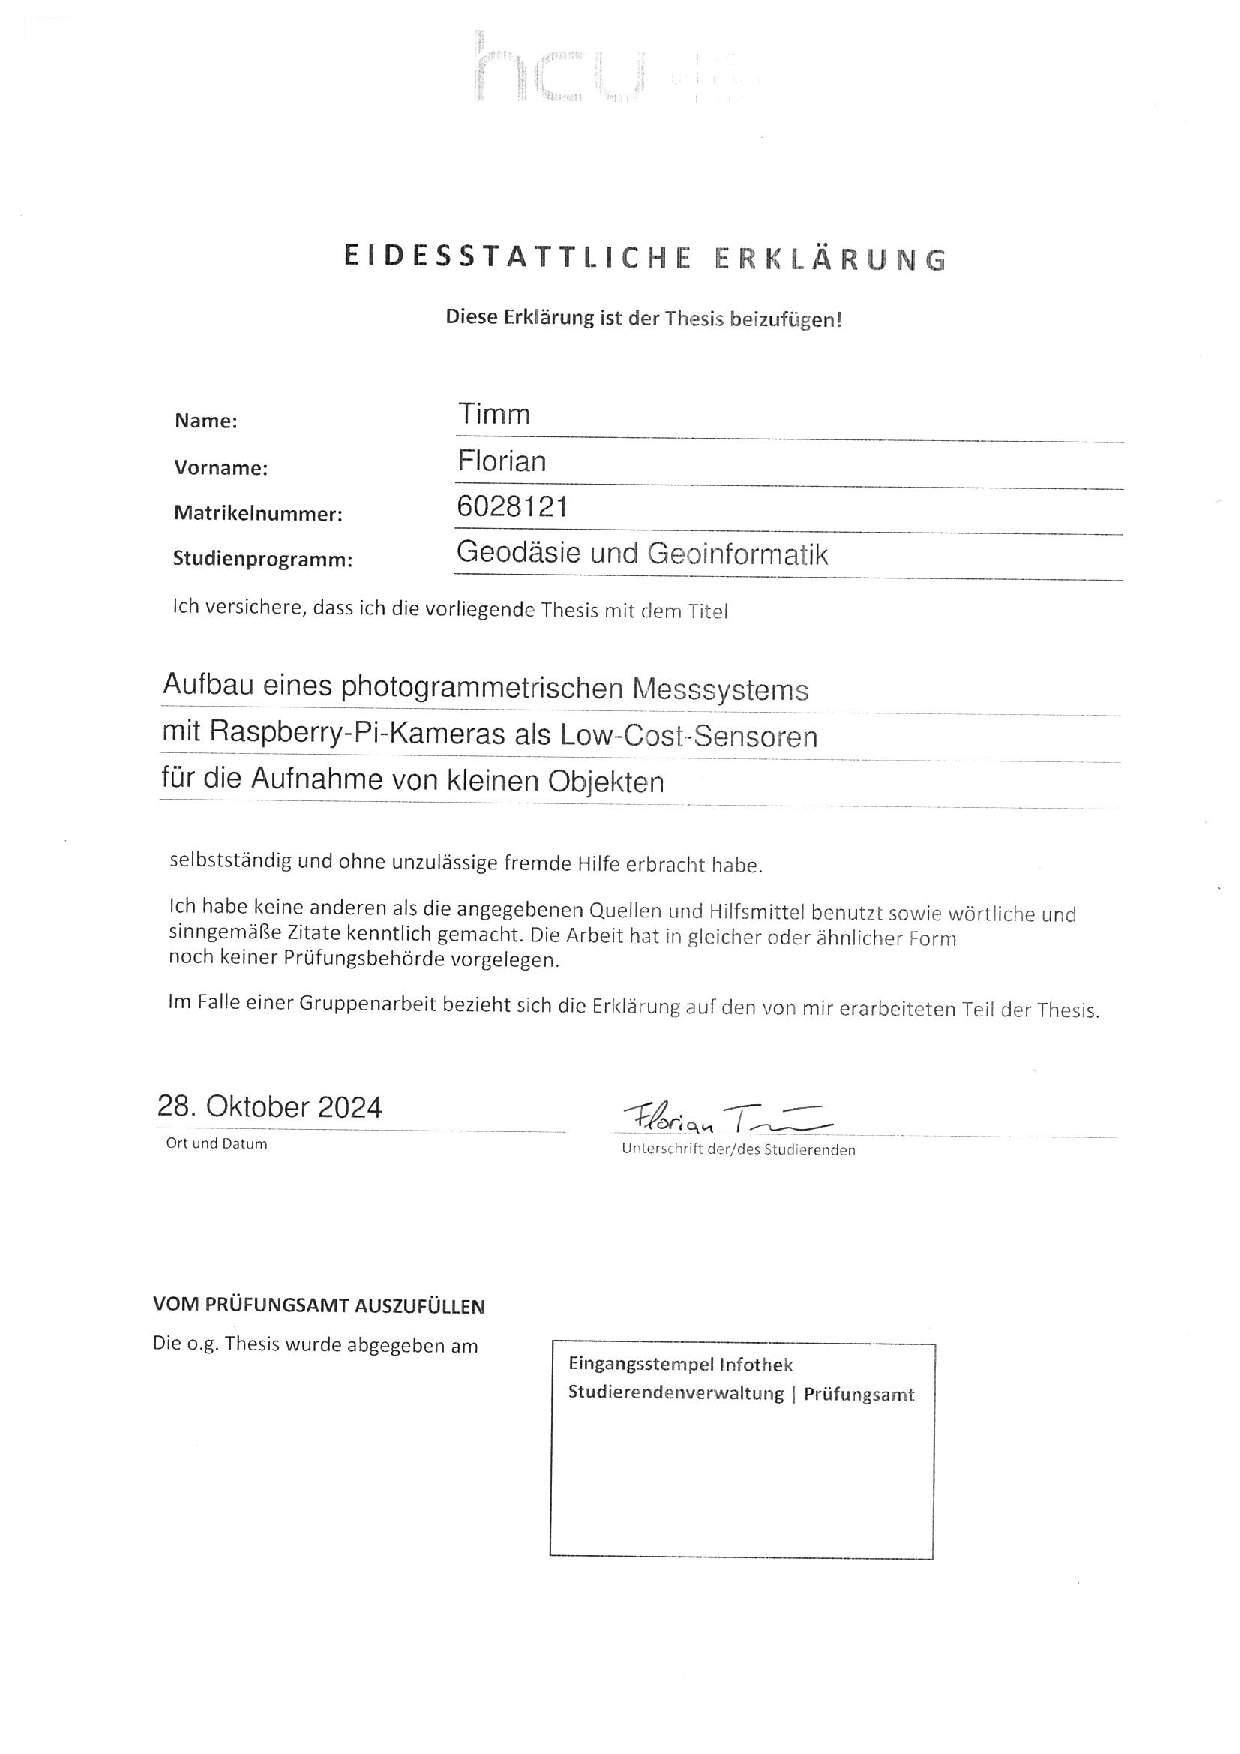
\includepdf{img/eidesstattliche_erklaerung.pdf}

\end{document}